\documentclass[11pt,a4paper,twoside]{article}

\usepackage[hmargin=2.7cm,vmargin=3cm]{geometry}
\usepackage{moreverb}
\usepackage{graphicx}
\usepackage{wrapfig}
\usepackage{expdlist}
\usepackage{svn}
\usepackage{fancyhdr}
\usepackage{extramarks}
\usepackage{color}
\usepackage[colorlinks=true,urlcolor=blue,linkcolor=blue]{hyperref}
\usepackage{ifthen}

\pagestyle{fancy}
\renewcommand{\sectionmark}[1]{\markboth{\thesection.\ #1}{}}
\renewcommand{\familydefault}{\sfdefault}

% Begin new paragraphs without indentation but vertical space.
\setlength{\parindent}{0pt}
\setlength{\parskip}{1.5ex plus 0.5ex minus 0.2ex}

% Setup framebox margin and frame rule size.
\setlength{\fboxsep}{0pt}
\setlength{\fboxrule}{0.6pt}

\newcommand{\DOMjudge}{\textsc{DOM}judge }

% Display commands, arguments, etc. in texttt font and don't break those.
\newcommand{\cmd}[1]{\mbox{\texttt{#1}}}

% Only show text if the submitclient is configured
\newcommand{\ifcmdsubmit}[1]{\ifthenelse{\equal{\SUBMITCLIENTENABLED}{yes}}{#1}{}}

% Our titlepage, should be called at start of team manual document
% Argument list:
% #1 - DOMjudge version
% #2 - Document revision
% #3 - Last modified date
% #4 - Generated date
% Also define the following words for language overrides:
\newcommand{\versionrevison}{Version/revision}
\newcommand{\lastmodified}{Last modified}
\newcommand{\generated}{Generated}
\makeatletter
\newcommand{\titlestuff}[4]{%

  \thispagestyle{plain}
  \vspace*{-2cm}
  \parbox[t]{\linewidth}{%
    \begin{wrapfigure}[1]{r}{2cm}
      \vspace*{-1cm}\hfill
      \includegraphics[height=4cm]{../logos/DOMjudgelogo.pdf}
    \end{wrapfigure}
    {\fontfamily{phv}\fontseries{b}\fontsize{26pt}{28pt}\selectfont \@title \par}
  }
  \vskip 2cm

  % Setup fancy headers/footers (here because we need SVN stuff defined)
  \def\setupfancystuff{%
    \fancyhead{}
    \fancyfoot{}
    \fancyfoot[RO,LE]{\thepage}
    \fancyfoot[LO,RE]{%
      \color[gray]{0.5}\vspace{-0.3cm}
        \DOMjudge team manual -- \generated: #4 \\
    }
  }

  % First for fancy page style:
  \setupfancystuff
  \fancyhead[RO,LE]{\slshape \firstleftmark}

  % No headers for plain page style (titlepage):
  \fancypagestyle{plain}{%
    \setupfancystuff
    \renewcommand{\headrulewidth}{0pt}
  }
}
\makeatother


\usepackage[dutch]{babel}

% Redefine words for date/versioning:
\renewcommand{\versionrevison}{Versie/revisie}
\renewcommand{\lastmodified}{Laatst gewijzigd}
\renewcommand{\generated}{Gegenereerd}

% For inclusion of the correct date (last modified) and revision.
% Use the \SVN command to get language dependent formatting of the
% date. We need to do some %/$ comment character magic to satisfy both
% TeX and 'git log' format string formatting both with and without
% expansion of the $Format$ keyword below with 'git archive'.
\SVN $Date: 1900-01-01 00:00:00 +0000 $
\SVN $Rev: unpublished $
% $Format:
%n\SVN %x24Date: %ai %x24$
% $Format:
%n\SVN %x24Rev: %h %x24$

\title{\DOMjudge teamhandleiding}

\hypersetup{
	pdftitle={DOMjudge teamhandleiding},
	pdfauthor={DOMjudge Developers: domjudge-devel at domjudge.org},
	pdfsubject={Instructie voor teams die de interface van het DOMjudge jurysysteem gebruiken tijdens een programmeerwedstrijd},
	pdfkeywords={DOMjudge,manual,team,handleiding,judge,jury,programmeren,wedstrijd,programmeerwedstrijd,icpc,acm}
}

\begin{document}

\titlestuff{\DOMJUDGEVERSION}{\SVNRev}{\SVNDate}{\today}

\section*{Samenvatting}

Hieronder staat de belangrijkste informatie kort samengevat. Dit is
bedoeld om snel aan de slag te kunnen. We raden echter ten zeerste
aan dat minstens \'e\'en iemand binnen je team de complete handleiding
doorneemt, omdat daarin specifieke details van het jurysysteem staan
die ook van belang kunnen zijn op het moment dat niet alles perfect
gaat. \textbf{WEES GEWAARSCHUWD!}

DOMjudge werkt via een web-interface die je kunt vinden op \\
\url{\WEBBASEURI team}. De figuren~\ref{fig:team-overview}
en~\ref{fig:team-scoreboard} op de volgende pagina geven een impressie
hiervan.

\subsection*{Inlezen en wegschrijven}

Oplossingen moeten invoer en uitvoer lezen van `standard in'
(toetsenbord) en wegschrijven naar `standard out' (beeldscherm). Je
hoeft dus nooit een bestand te openen. Zie bijlage~\ref{codeexamples}
voor een aantal voorbeelden hiervan.

\subsection*{Insturen van oplossingen}

Insturen van oplossingen gaat via%
\ifcmdsubmit{ het command-line programma \cmd{submit} dan wel}
de web-interface:
\begin{description}[\breaklabel\setlabelstyle{\bfseries}]
\ifcmdsubmit{
\item[Command-line]
Gebruik \cmd{submit <bestandsnaam>}. Als je bestandsnaam de vorm
\cmd{<probleem>.<extensie>} heeft, met \cmd{<probleem>} het
label van het probleem en \cmd{<extensie>} een standaard-extensie van
de programmeertaal, dan worden deze automatisch gedetecteerd. Voor de
complete documentatie en alle opties, zie \cmd{submit --help}.
}
\item[Web-Interface]
Vanaf je teampagina op \url{\WEBBASEURI team} kun je een bestand
selecteren met de \textbf{Select file\ldots}-knop in de linker kolom en deze met
de \textbf{submit} knop insturen.
Standaard wordt het probleem uit het deel van de bestandsnaam v\'o\'or de
punt gehaald en de programmeertaal uit de extensie. Je kunt meer
bestanden toevoegen met de knop \textbf{Add another file}.

\end{description}

\subsection*{Bekijken van scores, inzendingen, e.d.}

Het bekijken van inzendingen, scores en sturen en lezen van
``clarification requests'' gaat via de web-interface in de rechter kolom.

\emph{Einde samenvatting.}

\begin{figure}[p]
  \centering
  \fbox{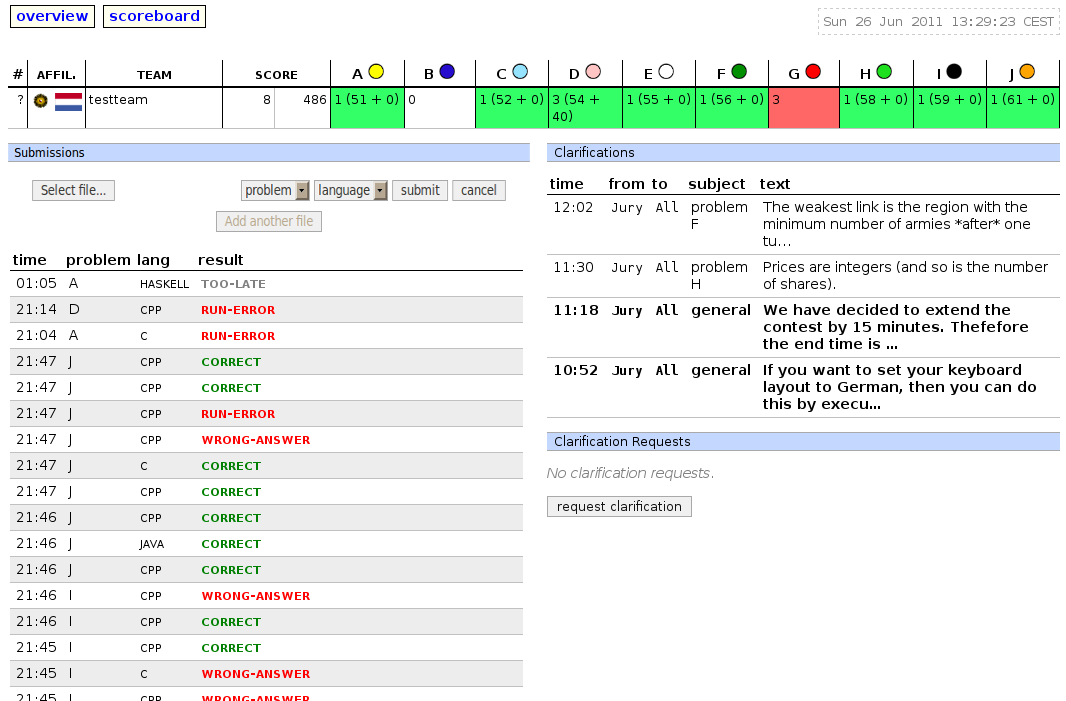
\includegraphics[width=15cm]{team-overview}}
  \caption{de team web-interface overzichtspagina.}
  \label{fig:team-overview}
\end{figure}

\begin{figure}[p]
  \centering
  \fbox{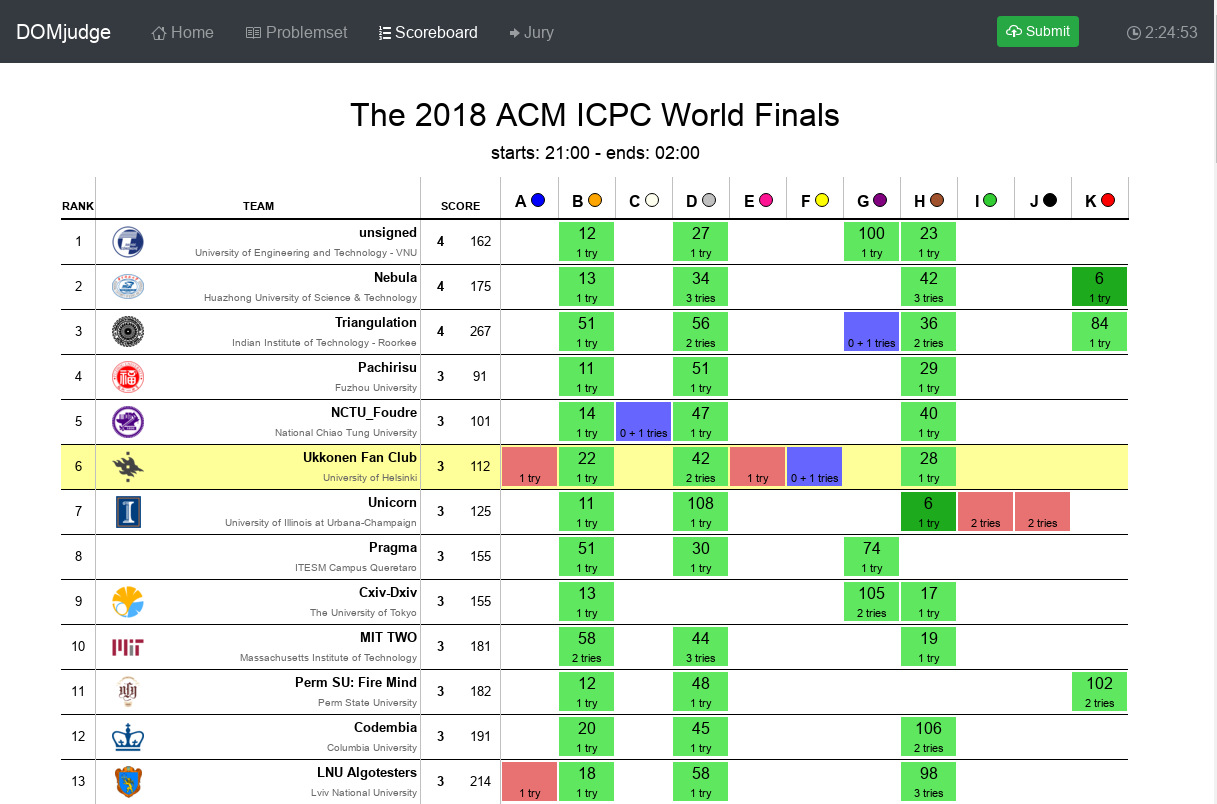
\includegraphics[width=15cm]{team-scoreboard}}
  \caption{de scorebord pagina.}
  \label{fig:team-scoreboard}
\end{figure}

\newpage

\section{Oplossingen insturen}\label{submit}

\ifcmdsubmit{
Het insturen van oplossingen voor problemen kan op twee verschillende
manieren: via een command-line interface (het programma \cmd{submit}),
of via de web-interface. Het kan zijn dat een van beide niet beschikbaar
is, afhankelijk van de configuratie van het systeem door de jury.
Hieronder worden beide methodes beschreven.

\subsection{Command-line: \cmd{submit}}

\textbf{Syntax:} \cmd{submit [opties] bestandsnaam.ext ...}

Het submitprogramma haalt de naam (label) van het probleem uit
\cmd{bestandsnaam} en de programmeertaal uit de extensie
\cmd{ext}. Dit kan handmatig aangepast worden met de opties
\cmd{-p probleemnaam} en \cmd{-l taalextensie}. Zie
\cmd{submit --help} voor een compleet overzicht van mogelijke
opties en extensies en een aantal voorbeelden. Als deze
helptekst niet op \'e\'en scherm past, gebruik dan
\cmd{submit --help | more} om alles te lezen.

\cmd{submit} zal het bestand controleren en eventueel
waarschuwingen geven, zoals wanneer het bestand al lange tijd niet
veranderd is of groter is dan de maximale source-code-grootte.
Bestandsnamen moeten beginnen met een alfanumeriek teken en
mogen daarna slechts bestaan uit alfanumerieke tekens en
\cmd{+.\_-}. Je kunt meerdere bestanden opgeven die deel uit
moeten maken van deze oplossing (zie sectie~\ref{howjudged}
`Hoe worden opgaven beoordeeld?').

Hierna geeft \cmd{submit} een kort overzicht met de details van de
inzending en vraagt om bevestiging. Controleer vooral of je het goede
bestand, probleem en taal hebt en druk dan op `y' om de oplossing in
te sturen. Als alles goed gaat, zal \cmd{submit} een melding geven
dat de inzending succesvol is. Indien niet, zal er een foutmelding
verschijnen.

Het submitprogramma maakt gebruik van een directory \cmd{\USERSUBMITDIR}
in de homedirectory van het account. Hier slaat het tijdelijk
bestanden op voor inzending en staat ook een logfile \cmd{submit.log}.
Verwijder deze directory niet en pas hem niet aan, omdat anders het
submitprogramma niet meer correct functioneert.
}

\subsection{Web-interface}

Vanaf je teampagina \url{\WEBBASEURI team} kun je oplossingen insturen
door het bestand te selecteren met de \textbf{Select file\ldots}-knop in de
linker kolom. \DOMjudge probeert het probleem te detecteren uit de
basis van de bestandsnaam (v\'o\'or de punt) en de programmeertaal uit
de extensie. Als dat niet lukt, kun je deze handmatig selecteren.
Bestandsnamen moeten beginnen met een alfanumeriek teken en
mogen daarna slechts bestaan uit alfanumerieke tekens en
\cmd{+.\_-}.

Nadat je de eerste bestandsnaam geselecteerd hebt, kun je extra bestanden
opgeven die deel uit moeten maken van deze oplossing door de knop \textbf{Add
more files} te gebruiken (zie sectie~\ref{howjudged} `Hoe worden opgaven
beoordeeld?').

Nadat je op de submitknop geklikt hebt en dit bevestigd hebt, word je
teruggestuurd naar de overzichtspagina. Daarop staat een
bericht dat je inzending succesvol ingestuurd is en zal de inzending
ook in lijst staan. Als er daarentegen iets misgegaan is, krijg je
daar een foutmelding over.

\section{De uitslag bekijken van inzendingen}

Op de team-webpagina staat in de linker kolom een overzicht van je inzendingen.
Dit overzicht bevat alle relevante gegevens: de tijd van inzending, de
programmeertaal, het probleem en de status. Hier vind je ook het scorebord
met de resultaten van de andere teams.

Bovenaan het overzicht staat de rij uit het scorebord van je eigen
team met je positie. Deze geeft al je opgeloste en geprobeerde
problemen weer. Je kunt het complete scorebord bekijken via het menu.
De meeste cellen op het scorebord geven extra details weer als ``title
text'' als je de muis erover houdt. De cellen in de score kolom geven
het aantal correcte opgaven en de totale straftijd weer. De volgende
cellen geven het aantal inzendingen voor ieder probleem. Als een
probleem succesvol is opgelost, dan staat erachter het aantal minuten
sinds het begin van de wedstrijd waarop de correcte oplossing
ingezonden is. Deze tijd telt mee voor de totale tijd, samen met een
straftijd voor alle voorgaande incorrect inzendingen.
Het scorebord kan mogelijk `bevroren' worden als het einde van de
wedstrijd nadert. Het scorebord wordt dan niet meer aangepast, maar de
rij op de overzichtspagina nog wel. Je positie wordt daar dan met een
`?' weergegeven.

\subsection{Mogelijke uitslagen}

Voor een ingestuurde oplossing zijn de volgende uitslagen mogelijk.

\begin{description}[\setleftmargin{4.5cm}]
\item[CORRECT]
Je oplossing heeft alle tests weerstaan: je hebt dit probleem opgelost!

\item[COMPILER-ERROR]
Het compileren van je programma gaf een fout. Bij de details
van deze inzending kun je de precieze foutmelding inzien
(deze optie kan uitgezet zijn).

\item[TIMELIMIT]
Je programma draaide langer dan de maximaal toegestane tijd en is
afgebroken. Dit kan betekenen dat je programma ergens in een loop
blijft hangen, of dat je oplossing niet effici\"ent genoeg is.

\item[RUN-ERROR]
Je programma gaf een fout tijdens het uitvoeren. Dit kan verschillende
oorzaken hebben, zoals deling door nul, incorrecte geheugen\-adressering
(segfault, bijvoorbeeld door arrays buiten bereik te indiceren), te
veel geheugengebruik, enzovoort.
Let ook op dat je programma met een exitcode 0 eindigt!

\item[NO-OUTPUT]
Je programma gaf geen uitvoer. Let op dat je uitvoer naar standard
output schrijft!

\item[WRONG-ANSWER]
De uitvoer van je programma was niet correct. Het kan zijn dat je
oplossing niet correct is, maar let ook goed op dat je de antwoorden
precies zoals beschreven uitvoert: de uitvoer moet exact kloppen met
de specificatie van de jury!

\item[PRESENTATION-ERROR]
De uitvoer van je programma verschilde slechts in presentatie
(bijvoorbeeld: de hoeveelheid witruimte) met de correcte uitvoer.
Dit wordt net als WRONG-ANSWER niet correct gerekend. Deze uitslag
is optioneel en mogelijk niet aangezet.

\item[TOO-LATE]
Helaas, je hebt ingestuurd nadat de wedstrijd al afgelopen was!
Je inzending is opgeslagen maar wordt niet verder behandeld.
\end{description}

\section{Clarifications}

Communicatie met de jury loopt door middel van \emph{clarifications}
(verhelderingen), deze komen in de rechter kolom op je teampagina te
staan. Boven aan de pagina de gegeven clarifications, daar onder je
\emph{requests} (verzoeken).

Je kan vragen aan de jury stellen door middel van het doen van een
``Clarification Request''; de knop hiervoor bevindt zich bovenaan de
clarifications kolom.  Je vraag zal alleen bij de jury aankomen; zij
zullen deze zo snel mogelijk en adequaat beantwoorden. Antwoorden die
voor iedereen relevant kunnen zijn zullen naar iedereen gestuurd worden.

\section{Hoe worden opgaven beoordeeld?}\label{howjudged}

Het \DOMjudge jurysysteem is volledig geautomatiseerd. Dit betekent
dat er (in principe) geen menselijke interactie is tijdens de
beoordeling. Het beoordelen gebeurt via de volgende stappen:

\subsection{Insturen}

Via%
\ifcmdsubmit{ het \cmd{submit} programma of}
de web-interface (zie sectie~\ref{submit}) kun je een oplossing voor
een opgave insturen, zodat hij ge\"upload wordt naar de jury. Let op
dat je de source-code van je programma moet insturen (en dus niet een
gecompileerd programma of de uitvoer van je programma)

Dan komt je programma in de wachtrij te staan, om gecompileerd,
uitgevoerd en getest te worden op \'e\'en van de jury-computers.

\subsection{Compileren}

Je programma wordt op een jury-computer onder Linux gecompileerd.
Alle ingestuurde sourcebestanden worden aan de compiler gegeven die
hier \'e\'en uit te voeren programma van maakt. Het als eerste
opgegeven bestand wordt beschouwd als de `main' source, voor talen
waarbij dat relevant is.

Als je een andere compiler of besturingssysteem gebruikt dan de jury,
moet dat in principe geen probleem zijn, maar let wel op dat
je geen compiler/systeem-specifieke dingen gebruikt (afhankelijk van
de configuratie kun je bij een compileerfout de foutmelding bekijken).

Binnen het jury-systeem worden \cmd{ONLINE\_JUDGE} en \cmd{DOMJUDGE}
gedefinieerd: als preprocessor symbolen in gecompileerde talen, als
(environment) variabelen in scripttalen.

\subsection{Testen}

Als je programma succesvol gecompileerd is, wordt het gedraaid en de
uitvoer vergeleken met de correcte uitvoer van de jury. Er wordt eerst
gecontroleerd of je programma correct ge\"eindigd is: als je programma
met een fout eindigt en het goede antwoord geeft, krijg je toch een
\textsc{run-error}! Er zijn een aantal beperkingen die aan je programma
opgelegd worden. Als je programma die overschrijdt, wordt het ook
afgebroken met een fout, zie sectie~\ref{runlimits}.

Verder moet de uitvoer van jouw programma exact overeenkomen met de
uitvoer van de jury. Let dus goed op, dat je de uitvoerspecificatie
volgt. In gevallen waarin er niet \'e\'en unieke uitvoer is (zoals bij
floating point-antwoorden) kan de jury een aangepaste beoordeling
hiervoor maken.

\subsection{Beperkingen}\label{runlimits}

Om misbruik tegen te gaan, het jurysysteem stabiel te houden en iedereen
duidelijke, gelijke omstandigheden te geven, zijn er een aantal
beperkingen die aan iedere ingestuurde oplossing opgelegd worden:

\begin{description}[\setlabelphantom{aantal processen}]
\item[compile-tijd]
Je programma mag er maximaal \COMPILETIME\ seconden over doen om te
compileren. Daarna wordt het compileren afgebroken en levert dit een
compileerfout op. Dit zou in de praktijk nooit een probleem mogen
opleveren. Mocht dit toch gebeuren bij een normaal programma, laat het
dan de jury weten.

\item[sourcegrootte]
De totale hoeveelheid sourcecode per ingestuurde oplossing mag
maximaal \SOURCESIZE\ kilobytes groot zijn, anders wordt je
inzending geweigerd.

\item[geheugen]
Je programma heeft tijdens het draaien maximaal \MEMLIMIT\ kilobytes
geheugen ter beschikking. Let op dat dit totaal geheugen is (inclusief
programmacode, eventuele virtual machine (Java), statisch en dynamisch
gedefinieerde variabelen, stack, \dots)! Als je programma meer
probeert te gebruiken, zal het afgebroken worden, zodat dit een
``\textsc{run-error}'' geeft.

\item[aantal processen]
Het is niet de bedoeling dat je programma meerdere processen (threads)
start. Dit heeft ook geen zin, want je programma heeft precies \'e\'en
processor volledig tot zijn beschikking. Om de stabiliteit van het
jurysysteem te bevorderen, kun je maximaal \PROCLIMIT\ processen
tegelijk draaien (inclusief de processen waardoor je programma
gestart is).

Mensen die nooit met meerdere processen geprogrammeerd hebben (of
niet weten wat dat is), hoeven zich geen zorgen te maken: standaard
draait een gecompileerd programma in \'e\'en proces.

\end{description}

\subsection{Java klassenaamgeving}

Het compileren van Java broncode wordt gecompliceerd door de
klassenaamgeving van Java: er is geen vast startpunt van de code;
iedere klasse kan een methode \texttt{main} bevatten. Een klasse die
\texttt{public} gedeclareerd is, moet verder in een bestand met
dezelfde naam staan.

In de standaard configuratie detecteert DOMjudge automatisch de
hoofdklasse. Anders moet de hoofdklasse ``\verb!Main!'' heten en een
methode ``\verb!public static void main(String args[])!'' hebben. Zie
ook het Java codevoorbeeld in appendix~\ref{codeexamples}.

\newpage
\appendix

\section{Codevoorbeelden}\label{codeexamples}

Hieronder staan een aantal voorbeelden van code om de invoer van een
probleem in te lezen en de uitvoer weg te schrijven.

De code hoort bij de volgende probleembeschrijving: 
De invoer bestaat uit \'e\'en regel met daarop het aantal testgevallen.
Daarna volgt voor elk testgeval een regel met daarop een naam (\'e\'en
woord). Print voor elke naam de string ``Hello $<$naam$>$!''. Een naam
is maximaal 99 karakters lang.

Dit probleem zou de volgende in- en uitvoer kunnen hebben:

\begin{tabular}{|p{0.47\textwidth}|p{0.47\textwidth}|}
\hline
\textbf{Invoer} & \textbf{Uitvoer} \\
\hline
\verbatiminput{../examples/example.in} &
\verbatiminput{../examples/example.out} \\
\hline
\end{tabular}

Let op dat het getal 3 op de eerste regel aangeeft dat er 3
testgevallen volgen.

Een oplossing voor dit probleem in C:
\listinginput{1}{../examples/example.c}

Let op de \cmd{return 0;} aan het einde, zodat we geen
\textsc{run-error} krijgen!

\newpage

Een oplossing in C++ kan als volgt:
\listinginput{1}{../examples/example.cc}

Een oplossing in Java:
\listinginput{1}{../examples/example.java}

\newpage

Een oplossing in C\#:
\listinginput{1}{../examples/example.cs}

Een oplossing in Pascal:
\listinginput{1}{../examples/example.pas}

En tenslotte een oplossing in Haskell:
\listinginput{1}{../examples/example.hs}

\end{document}
